%%
%% VERSION HISTORY
%%    22 May 2006 - John Papandriopoulos - Original version
%%    12 Jul 2007 - John Papandriopoulos - Converted into template
%%

\chapter{Literature review}
	\label{chapter:a-new-hope}
	%

% preferred location for figures in this chapter
\setfigurepath{figures/chapter-2}

%=========================================================================

\iffalse
\begin{synopsis}
	In this chapter...
\end{synopsis}
\fi
%=========================================================================
\section{Types and process of suicide}

\subsection*{Types of suicide}

Suicide is defined as act of a person has self-awareness and intentionally engages in effort to end his or her life. In other word, suicidal behaviour is any active or passive acts initiated by a person with expectation to cause self-inflicted deatch. Emile Durkheim, a French sociologist specified four different types of suicide \cite{Durkheim1897}, they are illustrated in Figure~\ref{fig:types_of_suicide}.\\
\begin{figure}[!ht]
\centering
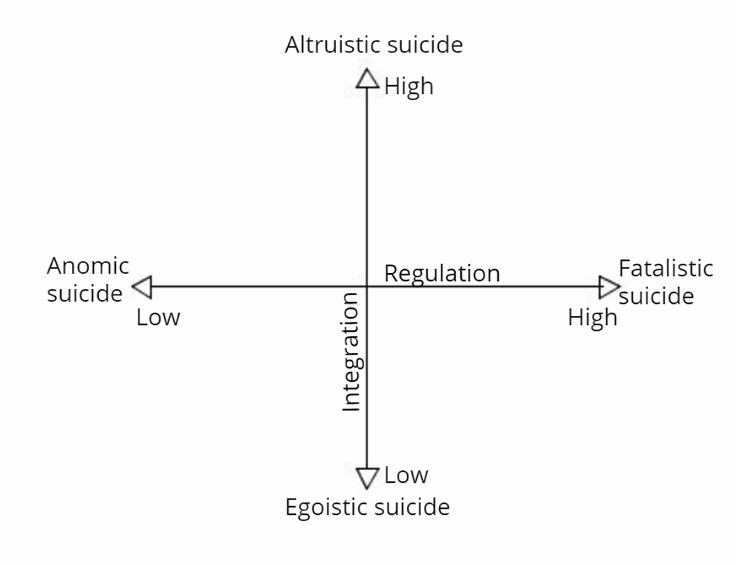
\includegraphics[width=\textwidth, clip=true]{img/type_suicide}
\caption[Types of suicide]{Types of suicide according to Émile Durkheim} 
\label{fig:types_of_suicide}
\end{figure}
(1) \textbf{Egoistic suicide:} It is a type of suicide occurs when an individual has low level of social integration. It means one does not feel he or she belong to or being accepted in a community. If this happens for a long time, it can lead to feeling of emptiness, melancholy and chronic depression. Those people feel isolated and receive little social support when they undergo hardship in life, leading to higher chance of committing suicide. It is called egoistic suicide because it springs from excessive individualism. To take example of this, Durkheim reported that the suicide rate among unmarried men is higher than that of married man since the unmarried are less bound and not connected to social norms.\\
(2) \textbf{Altruistic suicide:} In contrast to egoistic suicide, altruistic suicide occurs in societies with high integration. When an individual is overwhelmed by a community's beliefs, he put his personal values lower than community's values as a whole and considers mutual interests of community is more important than his needs. Examples for this type of suicide are suicide bomber and Samurai from Japan. Suicide bombers believe their death contribute to progress of his group to a common goal. In Samurai's code of feudal Japan, a Samurai who fail to complete an assigned task or lose in battle is seen as disgrace thus a samurai commits suicide when he feels humiliation and dishonored.\\
(3) \textbf{Anomic suicide:} Anomic suicide takes place in society with low degree of regulation. In a situation of sudden economic and social turmoil, an individual may question his morality due to lacking of social direction and deregulation of social ethic. People get frustrated when they fail to realize their desires and are being disappointed by it constantly. An example of this is suicide rate surges when there is a economic upheaval, crash of stock market or bankruptcy.\\
(4) \textbf{Fatalistic suicide:} Opposite to anomic suicide, fatalistic suicide happens when people are kept under tight regulation. An overregulated society has extreme rules and discipline, making its inhabitants feel suffocated by high standard and expectation. These people would prefer death to living within such harsh environment. Typical example of this kind of suicide is students under pressure of academic performance set by parents or their teachers.\\

\subsection*{Process of suicide}
According to authors of \cite{O'Carroll1996}, suicidal ideation refers to an individual's rumination about conducting suicidal behaviour. Suicide plan includes idea about time, location and method of suicide. Suicide attempt is a self-initiated, self-inflicted and injurious act following suicide plan performed in order to end one's life.\\
Figure~\ref{fig:suicide_process} shows the process of suicide. Suicidal ideation is first phase, where thought of suicide appear with possibly a statement or threat of suicide. Suicide plan precedes actual suicide attempt, it is characterized by suicide rehearsal which is behavioral enactment of a lethal method for suicide.\\
It is important to identify suicidal ideation because taking action early may stop progression of suicide process. Therefore, spotting suicidal ideation is vital and should be top priority in suicide prevention.
 
\begin{figure}[!ht]
\centering
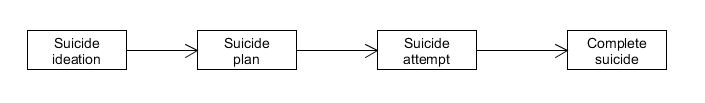
\includegraphics[width=\textwidth, clip=true]{img/suicide_process}
\caption[Process of suicide]{Flow diagram of suicide process} 
\label{fig:suicide_process}
\end{figure}

\section{Emotion classification in suicide notes}
Although the research of suicidal text started in 1960s with linguistic analysis of suicide notes to distinguish between genuine and stimulated notes, the application of NLP and ML in the same task appear in 2010 \cite{Desmet2013}. Pestian et al \cite{Pestian2010} applied ML algorithms to differentiate the notes of suicide completer and notes written by healthy control group and compared the accuracy of classifiers to accuracy of mental health providers. The best algorithm obtained the accuracy of 78\%, exceeding human professionals accuracy by 13\%. This promising result laid the foundation of NLP techniques on suicide notes. It also suggests the potential possibility of computer assist human in assessing suicide risk. However, the sample size for the study is only 66 and is derived from old study which reduce the reliability since the machine focus on the structure of the notes rather than content like what human usually do.\\
In 2011, the competition i2b2 NLP Challenge\footnote{https://www.i2b2.org/NLP/Coreference/} attracted 106 scientists from 24 teams to solve a shared task \cite{Pestian2012}. Track 2 of the challenge require participants to classify sentences in suicide notes in one or more of 15 categories which are 13 emotions: love, guilt, fear, hopelessness, forgiveness, sorrow, anger, abuse, blame, happiness, peacefulness, thankfulness, pride  and 2 non-emotion classes namely instruction and information. The training set is 600 actual suicide notes collected by Dr. Edwin Shneidman and Cincinnati Children Hospital Medical Center and 300 other notes were use as test set and released after the challenge ended. The notes are labelled by different volunteers recruited online. Unlike crowdsourcing, these volunteers are not chosen randomly but were purposely contacted directly via email or indirectly by announcement on Facebook groups. Therefore, they have some emotional connections to suicide topic. The researchers sent e-mail to approximately 1500 members of some online suicide support groups and announced the study on Facebook suicide bereavement pages. Respondents must meet some criteria: over 21 year of age, primary language is English and willing to annotate 50 notes. After that, they will be asked for general information like relationship to the lost person, how long it has been, and presence of symptoms of mental illness before suicide. They gained access to website to do the annotation task online. Only annotators that have 50\% agreement rate or more with gold standard after the first 10 training notes can continue to label 50 notes more. The characteristics of annotator is summarized in Table~\ref{tab:annotator}.
\begin{table}
\noindent\begin{tabularx}{\textwidth}{ll}
\midrule
Respondents who completed the training task     &    169   \\
Respondents who completed the full task            &     64   \\
Male                                                                       &     10\%   \\
Female                                                                  &     90\%  \\
Average age (standard deviation)                        &    47.3 (11.2)  \\
High school diploma                                              &   26  \\
Associates degree                                               &    13  \\
Bachelor's degree                                                   &    23  \\
Master's degree                                                   &     34  \\
Doctoral degree                                                 &    4  \\
\bottomrule
\end{tabularx}
\caption{Characteristics of annotators}
\label{tab:annotator}
\end{table}
Each team is allowed to submit at most three systems thus some teams have similar strategies: develop two classifiers and "combine" them into a hybrid classifier. Wang et al \cite{Wang2012} developed a ML classifier using support vector machine (SVM) along with one-against-one approach for multi-label classification. Before training the data, they pre-processed data to aim for betting parser accuracy and give similar meaning to syntactically different expression. For example, they correct misspellings, normalize symbol and number (’+’ to ’and’, ’\$100’ to ’\$MONEY\$’). Their second system is a rule-based classifier that create set of patterns from training data automatically and using $\chi^2$ test and choose a fixed number of pattern sets to reduce pattern space. A notion called g-measure was defined, it is a conditional probability of sentence that contain a specific pattern belong to a specific class. The highest g-measure is chosen for that categories to be labelled for a sentence if it is higher than a specific threshold. The team has experimented to find threshold that produce highest F-score and choose it to be fixed threshold for hybrid system. A simple combination rule is used to form a hybrid classifier: if a sentence is not labelled by SVM classifier, then result of rule-based classifier is assigned to that sentence. The threshold approach gives better precision (often higher than 0.6) than recall (lower than 0.4) since there are some sentences with various emotions in them and the threshold overlook low occurrence emotion.\\
Similarly, Sohn et al \cite{Sohn2012} proposed a ML system and a rule emphasis system. They used Weka\footnote{https://www.cs.waikato.ac.nz/ml/weka/} (Waikato Environment for Knowledge Analysis) and its multinomial Naive Bayes feature to create the ML system. Some techniques are applied in the process namely token normalization (e.g. "can’t", "ca n’t" convert to "cannot"), classifier ensemble (using different values for a parameter) and corpus-reannotation. Their rule-based system simply utilizes Perl regular expressions to match defined patterns. Again, hybrid system combines the result of the two systems to get the final label. They have more balanced result between precision and recall with both are in range 0.5 to 0.6. They also have data pre-processing with popular methods like symbol normalization using regular expression and post-processing phase. A shortcoming of this paper is lack of deep syntactic analysis making some rare classes (sorrow, forgiveness, abuse) did not occur at all. Another improvement can be made by analyze the effect of combining two systems, why it only improves the F-score just a tiny bit compared to other systems.\\
Luyckx et al \cite{Luyckx2012} approached the problem with a new way as they pre-process the data then carry out two processing phases: calibration and thresholding. In the pre-processing step, they tried to divided multi-labelled sentences into single-labelled fragments. If the sentence cannot be divided, then it would be discarded from training data. The calibration phase use SVM classifier with ten-fold cross-validation scheme on output of pre-processing step and evaluate lexical features, context features and lexicon-based features. The lexical features include some frequently occurred word that associated with a specific emotion (e.g. "can’t", "tired" for hopelessness). The context features consider the label of preceding and following sentences while lexicon-based features make use of a vocabulary of emotion. The thresholding phase applied various threshold to LibSVM (a learning package) probability estimates. In term of F-score, out of these three group, Union system of Sohn's group attained highest score of 0.5640 followed by 0.5038 and 0.5018 of Wang's team and Luyckx's team respectively. The mean performance of all team is 0.4875 with the median of 0.5027. The team with highest score achieve F-measure of 0.6139. The differences between these systems are summarized in Table~\ref{tab:teams}.\\


\begin{table}
\small
\noindent\begin{tabularx}{\textwidth}{llXXX}

\toprule
                    & Micro F\textsubscript{1}        &   Multi-system                              &  Learning algorithm            &   Feature engineering\\ 
\midrule
Sohn's team &  0.5640                & Yes (ML, rule-based and hybrid) &  Multinomial naive Bayes    &  Named Entity Recognition, n-gram tokenization, token normalization \\
Wang's team&  0.5038                & Yes (ML, rule-based and hybrid) & one-against-one SVM        &   n-gram tokenization, POS tagging, sentiment analysis\\
Luyckx's team&  0.5018              & No                                                & one-vs-all SVM                   & Multi-label training sentences re-annotated into single-label instances, unigram tokenization\\	

\bottomrule
\end{tabularx}
\caption{Comparison between teams: each team take different approaches, learning algorithm and feature engineering method}
\label{tab:teams}
\end{table}


Although all three teams have done some pre-processing steps but only Sohn's team do post-processing part to eliminate misclassified cases such as salutation being labelled instruction. They also used different learning algorithm from other teams (Naive Bayes vs SVM). This can be one of the reasons why they have smaller difference between precision and recall compared to their counterpart. Naive Bayes is usually work well on small text collection. Unfortunately, Luyckx's team could have achieved better result if they did not re-annotate the data. They chose to re-annotate because it shows promising result in the development phase but it turn out not good as they expect with F-score of 0.5018 while intact data could give them 0.5230 with roughly the same precision and recall (0.53 and 0.5 respectively). In these papers, the teams use standard, well-known methods in NLP and off-the-shelf packages to implement their systems, and it is not surprise since this challenge aim is to apply techniques to problem, not investigating pure theory. The challenges and workshops like i2b2 NLP Challenge inaugurate a specific task and
provide approaches to research community, promoting good solutions to be considered for similar tasks.\\

\section{Analysis of suicide with social media data}

Another research trend is using social media data to relate blog posts and suicide cases. Huang et al \cite{Huang2008} collected blog entries from MySpace.com and use dictionaries containing suicide-related keywords to detect blogs with suicidal intention. The study is one of the first to use social media data to find suicidal thoughts and that, in turn, set the new goal for NLP in the mental research: identifying mental suffering victims actively using social network and are at brink of suicide. Unfortunately, MySpace lost its popularity lead to researchers switching to other social networking sites for their study and finding the keyword is a primitive approach for a NLP task.\\
\subsection{Predicting national suicide numbers with social blog posts}
South Korea has the second highest suicide rate in the world (29.1 per 100,000), that make it the highest suicide rate in OCED countries (Organisation for Economic Co-operation and Development) \cite{Yoon2015}.Won et al \cite{Won2013} build a model to predict to suicide number in South Korea. The research team collected suicide data from January 1\textsuperscript{st} 2008 to December 31\textsuperscript{st} 2010. Their model considers social media data in form of suicide weblog posts and dysphoria weblog posts (blog entries containing specific words relate to suicide or dissatisfaction with one’s life), economic and meteorological data which are Korea Composite Stock Price Index (KOSPI), consumer price index (CPI), unemployment rate, temperature and sunlight hours of Seoul. Another interesting features is celebrity suicides, they also have quite strong correlation with number of suicide cases in corresponding month. The dataset is split into two sets: training set with data in two years 2008-2009 and validation set with data of 2010. They calculate numbers for 3-day epochs instead of taking daily numbers for each features. For example, suicide count feature is total number of suicide cases nationally over the time period of three days while the temperature features are average temperature over the course of three days. The researchers defined celebrity suicide for this paper as suicides emerge on three pre-eminent national television channels (SBS, KBS and MBC). There are 6 cases match the definition, 5 out of 6 people were actors or actresses and the remaining case was former President. Univariate linear regression model is used on each candidate predictors mentioned above to check whether they are statistically significant (P-value \textless  0.05) or not. The analysis excludes two variables namely CPI and unemployment rate. It is surprise that unemployment rate is ruled out since unemployment is thought as one of causes of depression, poverty and suicide. The final model attained the adjusted R-squared value of 0.66, prediction accuracy of 0.79 and correlation of 0.74 on validation set (96/121 epochs). A second sensitivity analysis without celebrity suicide without the celebrity suicide variable was performed as the variable only fit short term trend. The accuracy increases to 0.83 but the correlation decrease by small amount 0.02. Won and his colleagues notice the dysphoria weblog count is a powerful predictor for actual long term number of suicide deaths. This study has confirmed association between digital social blog posts and national suicide data and pointed out possibility of using predictive model for suicide research on a large scale. \\

Later in the USA, Jashinsky et al \cite{Jashinsky2014}  investigated the suicide risk factors via Twitter data. They collected tweets (small blog entry with 140 characters restriction) with official Twitter application programming interface (API). The API allows users to retrieve tweet in a specific period of time with some available criteria such as keyword. They created a list of filter term to identify high concerning entries and attempted to remove the entries with joke, sacarstic intention. The result shows there is correlation between observed Twitter data with data obtained from real world suicides in states with highest suicide rate such as Alaska, New Mexico and Idaho. Both studies focus on public blogs containing keywords and actual number of suicidal deaths but there are differences between them: sample data duration range (3 months vs 3 years), geolocation (each states vs whole nation), number of variables. This research suggesta it is a good idea to incorporate social media data into model that inspect suicide trend across geographic regions but more filter must be developed to get messages of real victim rather than relying on keywords in blog.\\

\subsection{Confirming Werther effect on social media}
Kumar et al \cite{Kumar2015a} investigated Werther effect of online forum. The term "Werther effect" refers to the phenomenom of increase in number of completed suicides and suicide attempt after reported case of celebrity suicides. The term is derived from the main character in the novel \textit{Die Leiden des jungen Werthers} (The sorrows of young Werther) by the famous German writer Johann Wolfgang von Goethe. Imitative suicidal behaviours follows well-known celebrity are "copycat suicides" where lethal means and method of suicide in a celebrity suicide case announced publicly on media are being used in suicide attempts. Kumar and his colleagues collected data on Reddit, a social media platform encompasses many subforums, each of those corresponds to a particular topic. Reddit provides an official API just like Twitter with various features including collecting posts, comments and metadata accompanied with them.\\
To collect data related to suicide, the researchers used API to collect posts from subforum r/SuicideWatch (SW - a suicide support forum) in time period October 16\textsuperscript{th}, 2014 - December 19\textsuperscript{th}, 2014. A total of 66,059 posts from 19,159 unique users was crawled. The way of identifying celebrity suicide in this study was different from that of the introduced work above \cite{Won2013}. They take suicide from a Wikipedia page listing celebrity suicides and get 10 suicides. To make sure those suicides are 'important' enough to cause Werther effect, a comparison of Wikipedia page view count of corresponding celebrity between two periods (2 weeks before and after) was conducted. The measure was converted to \textit{z}-score, 9 out of 10 suicides show positive change in \textit{z}-score thus being incorporated in the model. \\
The hypothesis to be tested in this study is whether or not there exists a surge in volume of posts of SW after a celebrity suicide. A baseline was established by choosing 20 consecutive two-week time period as pairs. These pairs must have no celebrity suicide in its time and starts in day of week. A set of control group comprises of 21 mental health (MH) subreddits is listed. The purpose is to determine the increase in posts of SW is caused by celebrity suicide but not by mental health problems. 32,509 posts from 23,807 unique users of MH subreddits were obtained. Content analysis in which linguistic measures, n-gram analysis and topic model analysis was carried out. The research team categorize linguistic features: affective attributes, cognitive attribute, linguistic style attributes and social attributes. The first and second category are measures derived from pschycholinguistic lexicon LIWC\footnote{http://liwc.wpengine.com/} (Linguistic Inquiry and Word Count) such as positive, negative affect, synonyms for set of cognitive and perceptive words like "see", "hear", "feel", "death". The third features are lexical density (words that have POS tag verb, noun, adjective, adverb), temporal reference (post, present, future tenses), social/personal concerns (words in topics of family, friend, work, home), interpersonal awareness (first person singular/plural, second and third person pronouns). Social attributes include metadata for a post: length of post, number of upvotes, downvotes and comments, average comment length. N-gram analysis involves log likelihood ratio of unigram, bigram and trigram between prior and post celebrity suicide. Topic model analysis runs Latent Dirichlet Allocation (LDA) \cite{Blei2003} to retrieve 50 topics and then calculate posterior probability of each topic for both items in each pair time period. The objective of this analysis is to measure the increase in topic by computing the difference between posterior probability of pre- and post-suicide.\\
The result of post volumne comparison is no surprise as mean change in \textit{z}-score of number of posts after suicide is higher than that of baseline and control group (3.64 compare to 1.95, 0.45). The results of statistical testing on linguistic features give insight of content between pre- and post-suicide time period. Post-suicide posts show more negativity in emotional expression, cognitive biases and lower lexical density. They also reveal SW users is more lingering to the past than interest in future. Besides they show little concerns over society but focus on their own self by using more first person singular. The n-gram analysis report more symptoms of depression, anxiety after celebrity suicide. Negative n-gram like “i hate it”, “i gave up”, “tired of living” rise in frequency post-suicide. \\
The work have verified the Werther effect in posting activity of a online forum. The increase of posting activity in suicide support forum after a celebrity suicide is not coincidence but follows a consistent pattern. However, we should be cautious when drawing inference from this study as we do not have sufficient evidence on how posting activity related to actual number of completed suicides or suicide attempt.\\

\subsection{Identifying at-risk individuals and suicidal thoughts on social media}
\subsubsection*{Analysis of Twitter posts before suicide attempters}
%\addcontentsline{toc}{subsubsection}{Twitter}
Coppersmith et al \cite{Coppersmith2016} explore the Twitter posts of suicide attempters to see whether or not their linguistic style is different after the attempt. The researcher crawled the Twitter data to identify people who have publicly disclose their suicide attempt and enough information for reader to infer the time of it. 554 users are found to had declared their suicide attempt, only 163 of them indicated the exact date and 125 users have data prior to their suicide attempts. To avoid situation in which users did not actually attempt suicide or they was joking with their friends, a human examined tweets to ensure three conditions: the attempts seems to be true as stated; users are talking about their own attempts, not attempts of other people; and time of the attempts can be determined.\\
Demographics of users gives information about age group and gender of suicide attempters. In the data, more women are present than men and almost all of attempts are in the age range from 15 to 29. This distribution do not follows Twitter demographics as middle age and adult users account for 12\% and 37\% of total number of users respectively. It is expected given the nature of social network usage in youth where youngsters are more active and open to share opinion online.\\
The linguistic characteristics of suicide attempters is compared to neurotypical group (control group). Token is the unit for comparison, token here refer to a single word, emoticon or symbol. An emoticon is defined as visual representation of a facial expression using punctuation marks, numbers and letters, usually written to express a person's feelings or mood. For example, ":D" denotes a big smile. Similarly, an emoji is a graphic symbol that represent an object or an facial expressions but offer more versatility than emoticon due to larger range of expression including weathers, animals, places and its integration in website/application interface. Emoticons and emojis are very useful features to capture users' emotion at the time of writing. Notable pattern is observed: control group use more emoticons and emojis, users often talk about suice after the attempt rather than before it, users' language is self-attentional prior to an attempt.\\
Preprocessing phase is quite straightforward, all usernames and website addresses are replaced by single tokens "@" and "*". For example "Check out this awesome site: https://theawesomesite.com powered by @username123 :)" would be "Check out this awesome site * powered by @ ! :)". Character \textit{n}-gram model with \textit{n = 1, 2..., 5} is used together with logistic regression to separate suicide attempters from matched users in control group. Figure~\ref{fig:roc_curve} taken from the paper \cite{Coppersmith2016} shows the ROC (receiver operating characteristic) curve of this classification task. A ROC curve illustrates the tradeoff between true positive rate (recall) and false positive rate to aid the decision making process for optimal model. At a single point, the classifier achieves 70\% recall with only 10\% false alarms. A report \cite{Kann2016} has shown statistics of suicide attempt in youth and we can expect 4-8\% of users aged 15-29 will or have tried to take their life at some time. That makes the number of neurotypicals is ten times more than the number of at-risk youngsters. Assuming a population of 1000 people within age range 15-29, we expect 40-80 people will attempt suicide but taking 60 as a single number for simplicity. If the classifier maintains its performance in the experiment, we can identify 42 (70\% of 60) of them and misclassify 94 (10\% of 940) attempters as neurotypicals. This false negative need more screening for better assessment.
\begin{figure}
\centering
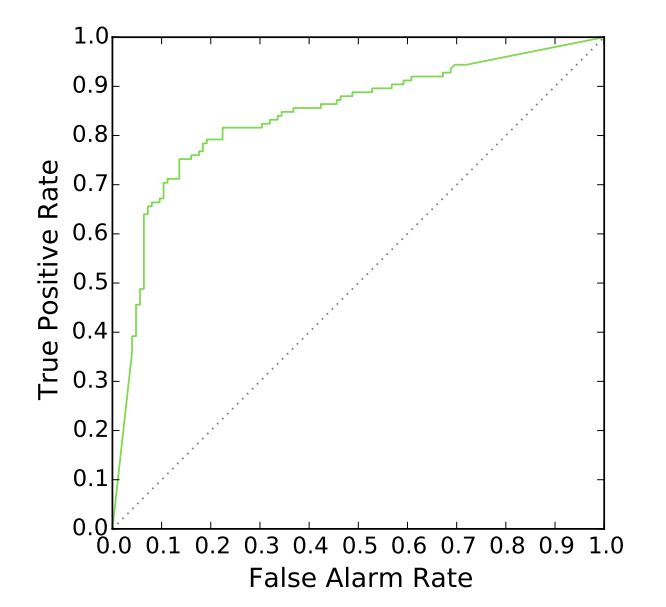
\includegraphics[width=\textwidth, clip=true]{img/ROC_curve}
\caption{ROC curve for separating users who attempted to take their life from matched neurotypicals \cite{Coppersmith2016}.} 
\label{fig:roc_curve}
\end{figure}
Although this study show some promising result in identifying at-risk individuals, the sample population is limited to female youngsters aged 15-29. This subpopulation of all age and gender group of Internet users is by no mean small. Howerver, generalizability of this method is not guarantee given characteristic of data in this paper.\\
% Classifying suicide communication content on Twitter
\subsubsection*{Classifying suicide communication content on Twitter}
While most studies are concerned about binary classification of suicidal intent, Burnap et al \cite{Burnap2015} explores the robustness of machine classification in a multiclass labelling task of Twitter posts where all classes are related to suicide but only one class shows suicidal intent. To define a list of terms to represent suicidal language, four websites with suicidal themes were selectied for crawling. These websites either have section\footnote{http://www.experienceproject.com}\textsuperscript{, }\footnote{http://www.enotalone.com} or are entirely dedicated to suicidal discussion\footnote{http://www.takethislife.com}\textsuperscript{, }\footnote{http://www.recoveryourlife.com}. 200 posts from each of these websites plus 1000 posts tagged with the word 'suicide' from popular microblogging site Tumblr\footnote{https://www.tumblr.com} were labelled whether this post is of suicidal person or not by human on crowdsourcing online service Crowdflower\footnote{http://www.crowdflower.com}. The labelled corpus was analyzed by applying Term Frequency/ Inverse Document Frequency (TF.IDF) process to \textit{n}-gram language model (\textit{n} = 1, 2,..., 5) at word level. Two experienced suicide researchers examined the top 500 terms from analyzing task to finally produce the list of 62 keywords that suggest possible suicidal ideation. Some examples of words in this list are "never wake", "kill myself", "don't want to exist". Over 4,000,000 tweets were crawled after applying suicided-related search terms in the time period  February 1\textsuperscript{st}, 2014 - March 15\textsuperscript{th}, 2014. Another set of search terms is proposed using name and surname of reported people die by suicide in England over the same period. The researchers sampled the two datasets to get random 1000 posts, 800 from the first dataset and 200 from 'names' dataset. Again, the same crowdsourcing service was used to classify posts into seven classes. Table~\ref{tab:class_of_comm} taken from the paper \cite{Burnap2015} gives description of classes. After removing tweets with low inter-rater agreement score computed by CrowdFlower (less than 75\%), 816 tweets remain to be used for ML classifier.
\begin{table}
\small
\noindent\begin{tabularx}{\textwidth}{>{\hsize=0.2\textwidth}X 
>{\hsize=0.5\textwidth}X  
>{\hsize=0.3\textwidth}X }

\toprule
Class & Description & \% of dataset\\ 
\midrule
C1  &  Evidence of possible suicidal intent & 13\\
C2 & Campaigning (i.e. petitions etc.)   & 5   \\
C3 & Flippant reference to suicide & 30  \\
C4 & Information or support & 6 \\
C5 & Memorial or condolence & 5 \\
C6 & Reporting of suicide (exclude bombing) & 15 \\
C7 & None of the above  &   26\\
\bottomrule
\end{tabularx}
\caption{Types of Suicidal communication with relative \% proportion in dataset \cite{Burnap2015}}
\label{tab:class_of_comm}
\end{table}
There are three feature sets in the experiment. Feature set 1 representing lexical characteristics of the sentences contain the following:
\begin{itemize}
\item \textit{Parts of speech}: frequency of each POS tag as a feature.
\item\textit{ Structural features}: inclusion of negations in the sentence, external communication link (URL, reply), usage of first person pronoun.
\item \textit{General lexical domains}: using Domains labels from Princeton WordNet\textsuperscript{\textregistered}\footnote{https://wordnet.princeton.edu/} (a large lexical database for English where words are grouped into sets of synonyms \cite{Fellbaum1998}, hereafter referred to as WordNet) to generate features represent categories such as home, psychology, etc.
\item \textit{Affective lexical domains}: include categories representing moods, emotional responses such as anger, sadness, love, hate, joy, etc.
\item \textit{Sentiments Score}: SentiWordNet\footnote{http://sentiwordnet.isti.cnr.it/} (a lexical resource for opinion mining based on WordNet) gives each word a score in interval [0,1] for negativity and positivity. The total score of all words in a tweets were used as features.
\item \textit{Frequent words}: The most used of unigrams, bigrams and trigrams in the training set.
\item \textit{Keyword list}: list of 62 keyword described above. 
\end{itemize}
Feature set 2 represents sentiment and emotional features. This set of features was compiled using LIWC to extract more lablels related to affective emotions in a tweets. These include term that have connection to topics causing distress like death, money, health, achievement, job. LIWC also have three categories frequently used in mental health research namely 'cognitive mechanisms', 'affect' and 'social words'. These mentioned features encompass feature set 2. Feature set 3 consists of regular expressions and pattern matching rules to match misspelled/shortened words. It is an attempt to recognize important phrases in a noisy and informal text environment due to number of character limit on Twitter. Some example phrases are "suicidal / cutting / bad / these ... thoughts / feelings", "want/wanted/wanting to die", "call/offer for/of help", "kill/killing/hate myself", "talk/speak to somone/somebody", "took/taken his/her own life". 
Three set of features was combined into one called combined set. Principal Component Analysis (PCA) was applied to the set to reduce dimension and retain sets of uncorrelated features (principal components). The text of tweets is transformed into word vector of uni-, bi- and trigrams and 500 words retained as features. The total number of feature is 1444.\\
Baseline was established using SVM, rule-based (Decision Tree - DT) and Naive Bayes (NB). All these three classifiers were used in an ensemple classifier called Roration Forest (RF). RF divides the feature set into smaller sets and run PCA on each set to generate principal components. These components is used to build classifiers. Ensemble meta classifiers produce out from multiple classifiers' output by using a voting mechanism. The voting rule here is choosing output with highest probability across all base classifiers. After some rounds of experiment running RF on the three baseline classifiers, the team dropped DT from the ensemble classifier, kept only SVM and NB in it.\\
Overall, the RF meta classifier using Maximum Likelihood voting mechanism with combined dataset achieved the best performance: precision = 0.732, recall = 0.729 and F-measure = 0.728. The key class of interest - suicidal ideation is inspected one more time and the RF model once again achieved highest recall (0.744) and F-measure (0.690) but not precision (0.644 while the highest being 0.657). Misclassification mostly occured in class 1 (suicidal ideation) and class 3 (flippant reference to suicide) indicating challenge posed by sarcasm and irony. Table~\ref{tab:confusion_matrix} taken from the paper \cite{Burnap2015} illustrates the confusion matrix of the best performing classification model on all seven classes.  
\begin{table}
\center
\small
\noindent\begin{tabularx}{0.5\textwidth}{cccccccc}
\toprule
Class & C1 & C2 & C3 & C4 & C5 & C6 & C7  \\ 
\midrule
C1  & \textbf{58} & 0 & 15 & 0 & 0 & 0 & 5\\
C2 & 0 &  \textbf{18} &  1 &  4 &  0 &  4 &  1 \\
C3 & 11 &  0 &  \textbf{143} &  0 &  1 &  5 &  17  \\
C4 & 0  &  4 &  5 &  \textbf{18} &  0 &  2 &  6\\
C5 & 1 &  1 &  1 &  0 &  \textbf{31} &  1 &  1\\
C6 & 0 &  6 &  9 &  7 &  2 &  \textbf{76} &  4 \\
C7 & 20 &  0 &  23 &  0 &  2 &  4 &  \textbf{94}\\
\bottomrule
\end{tabularx}
\caption{Confusion matrix for the best performing classification model \cite{Burnap2015}}
\label{tab:confusion_matrix}
\end{table}
This research explore the approach of using ensemble meta classifier to identify suicide-related communication on social media. If previous introduced work only interest in binary classification of suicidal and non suicidal posts, this one expand the scope the task. Multiclass labelling task can be useful in a broader context when other suicide-related messages may help automatically recognize news, reports, campaigns. Incorporating such classifier is beneficial for general-purpose crawling system. Although this study use some techniques specifically for Twitter, the main idea is likely applicable to other social media sites as well. 
%\subsubsection*{Reddit}
%\addcontentsline{toc}{subsubsection}{Reddit}
\subsubsection*{Identifying individuals who develop suicidal ideation on Reddit}
Another prominent social media site is Reddit\footnote{https://www.reddit.com/}. Reddit is one of the best sites for researchers because all the data is publicly available and development team even provides official API with many functionalities including collecting posts and comments. De Choudhury et al \cite{DeChoudhury2016} presented a statsistical methodology to identify individual who likely to discuss suicidal ideation given disclosure of their mental health earlier on Reddit. The research team collected posts and comments data from suicide support subreddit r/SuicideWatch (SW) and 14 mental health (MH) subreddits. All the posts and comments are in the time period February 11\textsuperscript{th}, 2014 - November 11\textsuperscript{th}, 2014. The size of content posted is considerable: 63,485 posts, 209,766 comments from 35,038 users of MHs and 16,348 posts from 9,224 users of SW. Two user classes are constructed for the classification task:
\begin{itemize}
\item \textbf{MH}: users who only posted on MHs in the first six months but never posted on SW in the last three months. 
\item \textbf{MH$\rightarrow$SW}: users who only posted on MHs in the first six months and posted on SW in the last three months
\end{itemize}
The process yielded 440 MH$\rightarrow$SW users and 28,831 MH users. To balance two classes, 440 users from MH were sampled randomly. The data reduced in sized accordingly: 4,731 posts, 46,949 comments from MH$\rightarrow$SW and 8,318 posts, 54,086 comments from MH. The prediction model adopted five sets of features: \textit{Linguistic structure}, \textit{Interpersonal awareness}, \textit{Interaction}, \textit{Content} and \textit{Full}. Automated readability index; percentage of nouns, verbs and adverbs; linguistic accommodation encompassed \textit{linguistic structure}. \textit{Interpersonal awreness} includes percentage of first person plural/singular, second and third person pronouns. \textit{Interaction} measures number of posts and comments each user had written, volume and length of comments received, mean score of posts and duration between post submission and the first comment to post. \textit{Content} features are all the unigrams and bigrams from posts and comments of both MH and MH$\rightarrow$SW. The \textit{Full} set is combined set of all four mentioned sets of features.\\
Some observations on difference between characteristic of MH and  MH$\rightarrow$SW give general impression about two cohorts. Firstly, MH$\rightarrow$SW users appear to display poorer linguistic structure and lower readability index. Secondly,  MH$\rightarrow$SW users is more self-focused and show little social concern by using first person pronoun more often than control group. Finally, MH$\rightarrow$SW users tend to have fewer posts but their posts are usually greater in length, indicating high degree of social isolation.\\
Content analysis entails causal inference. The authors chose propensity score matching to identify tokens that increase the likelihood of posting on SW. The tokens obtained make sense intuitively and increase the probability by 30-53\%. Some examples of these tokens are "useless", "anxiety", "no friends", "have nothing", "to cry". In contrast, some tokens decrease the likelihood on SW: "counseling", "intimate", "hope it", "and enjoy" significantly reduce the chance by 50-57\%. Besides identifying treatment tokens,  De Choudhury and her colleagues proceeded to link these tokens to specific themes and normalized spectral clustering algorithm was used. The algorithm maps the original space of similarity values to eigenvectors of a Laplacian matrix and applies standard clustering method (e.g. k-means). Six dominant themes corresponding to the first 6 eigenvalues of the matrix. Two researchers with experience on mental health content of social networking sites coded these 6 clusters of tokens and achieved high agreement rate (Cohen's $\kappa$ = 0.74). The six themes and some example tokens are:
\begin{itemize}
\item \textit{Hopelessness}: "have nothing" , "no real", "kill myself", "abandoned", "die".
\item \textit{Anxiety}: "anxiety", "panic", "to cry".
\item \textit{Impulsiveness}: "ending", "freaking out"
\item \textit{Self-esteem}: "hate it", "giving up".
\item \textit{Loneliness}: "my friends", "my parents", "alone".
\item \textit{Severe or stigmatized illness}: "depression", "psychosis", "disorder".
\end{itemize}
The main point of the study is the supervised learning task of predicting and classifying MH$\rightarrow$SW users from MH users. The train/test ratio is 80/20 and users classes in each set are balanced (704 users for training set plus 176 users for held-out validation set). The ML classifier used is regularized logistic regression. 10-fold cross validation is perform on the training set to tune parameters of all five sets of features. To reduce randomness of cross validation, the team run the models 10 times and reported the result that is most fitted to the data. Performance of the best model (\textit{Full}) on held-out set is reported in Table~\ref{tab:classifier_performance}.\\
\begin{table}
\small
\noindent\begin{tabularx}{\textwidth}{X|X|X|X}
Actual/Predicted & Class 0 & Class 1 & Total\\ 
\toprule
Class 0 & 73 & 15  & 88\\
Class 1 & 20 &  68 & 88\\ 
\midrule
Accuracy  & 83.5\%  & 77.5\% & 80\% (mean)\\
Precision & 0.79  &   0.82  & 0.81   (mean)\\
Recall     & 0.83   &    0.78   & 0.81 (mean)\\
F-1        &    0.81  &  0.80     &  0.80(mean)\\
\bottomrule
\end{tabularx}
\caption{Classifier performance distinguishing MH$\rightarrow$SW and MH \cite{DeChoudhury2016}.}
\label{tab:classifier_performance}
\end{table}
There are several limitations in this study. First of all, there may exists self-selection biases as Reddit does not enforce one account per user policy thus a user can have throwaway account, where user use an account to post in particular topics then abandon it, or register multiple accounts. Therefore, a person who intrinsically belongs to  MH$\rightarrow$SW may get excluded if he or she uses another account other than the main one to post in SW. Furthermore, we see imbalance between size of MH and MH$\rightarrow$SW and the authors decided to sample MH. This method shows robustness of the classifier in theoretical scenario but cannot ensure effectiveness in a larger population. 
%\subsubsection*{Reddit}
%\addcontentsline{toc}{subsubsection}{Reddit}
\subsubsection*{Analysis of commentary related to suicidal ideation on Reddit}
Following the previous study, De Choudhury and Kiciman \cite{DeChoudhury2017} continue to assess the impact of online social support in suicidal ideation. Data collection method is the same but now the focus shifts to comments received instead of posts from at-risk individuals. The dataset contained 62,024 comments from 32,362 users for 440 MH$\rightarrow$SW users and 41,894 comments written by 21,358 users for 440 MH users. All comments are tokenized, stopword removed and timestampt attached, into \textit{n}-gram tokens (\textit{n} = 2). Comment-tokens in a user's timeline is considered \textit{treatment} to that user. Post- and comment-tokens occur before a \textit{treatment} are \textit{covariates}. According to the terminology, a \textit{treatment group} is a group consists of users who received \textit{treatment} and a \textit{control group} characterized by users who have not encountered \textit{treatment}. Stratified propensity score maching is a statistical method to estimate the effect of a treatment from confounding covariates. The treatment group and the control group are treated as one big group and are divided into strata in which covariates of treatment subgroup and covariates of control subgroup are homogenous statistically. In this case, the dataset is stratified based on propensity score of receiving a particular treatment. Estimated propensity score is likelihood of receiving a treatment given covariates and it is calculated by a machine-learned function. To learn a propensity function, researchers applied averaged perceptron algorithm on vector \textit{H = h\textsubscript{1}, h\textsubscript{2}..., h\textsubscript{n}} where \textit{h\textsubscript{i}} is a binary variable that flags 1 if token \textit{i} appears before the treatment token and flags 0 otherwise. The treatment tokens are tokens that appear in more than 10 users' timeline of MH subreddits, the total number of treatment tokens is 11,278. The dataset is divided into 10 strata.\\
To ensure the strata is balanced, meaning users of both treatment and control groups are having similar effect when receiving comments, two human raters are employed. One is an expert in mental health content on social media sites and the other is a mental health professional. 150 treatment tokens with highest and lowest \textit{z}-score were chosen. Examples of negative treatment effect tokens (increase likelihood of being in MH) are: "lucky", "a reasonable", "enjoys", "gently", "heart and"; positive treament effect tokens ((increase likelihood of being in MH$\rightarrow$SW): "pain and", "not easy", "struggled", "hating". The human raters' task is to mark the similarity (0 or1 where 1 indicates high similarity) of 300 post pairs where a post pair consist of one post from treatment group user and one post from control group user. The agreement rate between two rater was high (Cohen's $\kappa$ = 0.81). This coding frame pinpointed which strata is balanced.\\
\begin{table}
\small
\noindent\begin{tabularx}{\textwidth}{>{\hsize=0.15\textwidth}X|XXXXXX}
\toprule
Feature & Count & Coverage & Effect & \textit{z}-val & $\chi^2$ & PMI\\ 
\midrule
gently &  43 &  0.3 &  -0.31 &  -2.18  & 2.55 &  0.02\\
sure of  & 43 &  0.49  & -0.22 &  -2.04 &  2.31 &  0.15\\
is helpful  & 37  & 0.49 &  -0.12  & -1.45  & 1.86 &  0.15\\
be tough  & 39 &  0.51  & -0.25  & -1.44  & 0.82  & 0.01\\
fight the  & 34  & 0.51 &  -0.23 &  -1.22  & 1.53  & 0.16\\
enjoyed it  & 46  & 0.3  & -0.18  & -1.1 &  0.71  & 0\\
be ready  & 39  & 0.49  & -0.04 &  -1.06 &  1.41 &  0.18\\
nice i &  54  & 0.39 &  -0.06  & -1.06  & 1.01 &  0.13\\
really fun &  35  & 0.2 &  -0.06  & -1.01 &  1.23 &  0.13\\
totally agree  & 37  & 0.49  & -0.05 &  -0.93 &  0.98  & 0.17\\
completed &  54 &  0.4 &  -0.09  & -0.91  & 0.25  & 0\\
enjoys  & 32 &  0.51 &  -0.08  & -0.85  & 1.23 &  0.18\\
defeat &  46 &  0.4  &  -0.28  &  -0.83 &  0.55 &  0\\
to defend  & 44 &  0.2 &  -0.08  & -0.79  & 1.18 &  0.14\\
was nice  & 37  & 0.49  & -0.12  & -0.77  & 0.97 &  0.1\\
really liked &  40 &  0.51  & -0.1 &  -0.61 &  0.88 &  0.08\\
be super  & 42 &  0.6  & -0.03 &  -0.54  & 1.38  & 0.17\\
instructions  & 54  & 0.39 &  -0.17  & -0.53 &  0.32 &  0\\
your home &  33 &  0.49 &  -0.11  & -0.45 &  0.55 &  0.08\\
kindness &  42 &  0.4 &  -0.11 &  -0.37 &  3.42 &  0.19\\
\midrule
proud  &  127 &  0.6 &  0.31 &  5.35 &  4.14 &  0.55\\
a hobby  & 35 &  0.49 &  0.53  & 4.87  & 4.57 &  0.76\\
am sorry &  34  & 0.49 &  0.53 &  4.77  & 4.69  & 0.77\\
suicide &  123 &  0.49 &  0.28 &  4.67  & 4.21 &  0.49\\
you wish  & 32  & 0.49 &  0.55 &  4.54 &  4 &  0.8\\
together with  & 32  & 0.49 &  0.51  & 4.54  & 4.16  & 0.72\\
medication &  114 &  0.49 &  0.35 &  4.51  & 4.13 &  0.56\\
friend you &  32 &  0.49 &  0.52  & 4.43  & 3.8 &  0.74\\
your opinion &  33 &  0.4  & 0.5  & 4.35 &  4.44  & 0.69\\
to respond &  40 &  0.49  & 0.49 &  4.34  & 3.41 &  0.69\\
i care &  40  & 0.4 &  0.55  & 4.31  & 4.57 &  0.81\\
depressed &  187  & 0.4  & 0.3 &  4.28  & 5.01 &  0.53\\
seek  & 132  & 0.39  & 0.27  & 4.26  & 4.41  & 0.47\\
pain and &  51  & 0.3 &  0.58 &  4.24  & 6.05  & 0.87\\
do well  & 44 &  0.4  & 0.56  & 4.11  & 4.32 &  0.82\\
stay strong &  48 &  0.4  & 0.52  & 4.09  & 4.16 &  0.74\\
medical  & 133 &  0.49 &  0.19  & 4.05  & 2.67  & 0.37\\
vent &  84 &  0.49 &  0.32 & 4.02 &  3.59 &  0.54\\
hating &  39  & 0.49  & 0.52  & 3.99 &  3.02 &  0.74\\
misery  & 34  & 0.49 &  0.5  & 3.96 & 3.13 &  0.7\\
\bottomrule
\end{tabularx}
\caption{Comment tokens given by propensity score matching that contribute to increased or decreased change in likelihood of being in MH$\rightarrow$SW or MH respectively \cite{DeChoudhury2017}.}
\label{tab:treatment_token}
\end{table}
Table~\ref{tab:treatment_token} taken from the paper \cite{DeChoudhury2017} shows 40 comment tokens with highest and lowest \textit{z}-score. The first half displays negative treatment tokens, the second half display positive treatment token. Coverage is percentage of users who belong to unclipped strata. PMI is the pointwise mutual information between the treatment token and the SW outcome (a user belongs to MH$\rightarrow$SW or not). Some tokens decrease likelihood of participating in  MH$\rightarrow$SW in the future by a significant percentage namely "gently", "sure of", "be tough", "fight the", "defeat". Whereas some tokens show very high positive treatment effect such as "suicide", "hating", "pain and", "am sorry".  
%\iffalse
\begin{table}
\small
\noindent\begin{tabularx}{\textwidth}{XX}
\toprule
Higher likelihood of being in MH &  Higher likelihood of being in MH$\rightarrow$SW\\ 
\midrule
\rowcolor{gray}
\textbf{Emotional Support}&\\
i \textit{totally agree}. It is hard. I have been there and it is not easy to handle the financial stress, buying a house, girlfriend being eight months pregnant, car issues, job issues, family issues. \textcolor{blue}{($\downarrow$5\%)}& I’ve recently lost friends whom I’ve known for 10 years, due to me being 'insensitive'. So yes sadly it does happen, I get you and what you are doing through. you are \textit{not alone}  \textcolor{red}{($\uparrow$16\%)}\\
\rowcolor{gray}
\textbf{Esteem Support}&\\
cheers mate, \textit{fight the} stigma, you can do it! \textcolor{blue}{($\downarrow$23\%)} & You have great potentials in self-actualizing your own situation and ending your \textit{misery}.  \textcolor{red}{($\uparrow$50\%)} \\
\rowcolor{gray}
\textbf{Informational Support}&\\
Ever thought of trying to find professional care? I suggest you do that. You need to give life a second chance it may surprise you a lot. I know it can \textit{be tough}, but worth it \textcolor{blue}{($\downarrow$25\%)}& If your issue is with the taking of \textit{medication}, talk to them about taking it, discuss your issues with it. Like the guy above said, it may help and could be worth a try, but it is good to discuss concerns about that sort of thing with the person prescribing it. \textcolor{red}{($\uparrow$35\%)}\\
\rowcolor{gray}
\textbf{Instrumental Support}&\\
Start by going for meditation. it can \textit{gently} help you break habitual negative thought patterns, and might also help you get a little bit of that "distance" from yourself that you are looking for \textcolor{blue}{($\downarrow$31\%)}& Bro, eat healthy, run, keep your room clean, actively suppress negative thoughts, force yourself to do something productive, even if it's just pursuing \textit{a hobby}. \textcolor{red}{($\uparrow$53\%)}\\
\rowcolor{gray}
\textbf{Network Support}&\\
There is no reason to be nervous and yet everyone here understands and have been precisely at the same place you are in your brave post. [...] i hope some of this discussion \textit{is helpful} to you. \textcolor{blue}{($\downarrow$12\%)} & Thats not true at all. everyone in this community really wants to hear your story. They would want \textit{to respond}. Everyones story is worth a listen don't you think? \textcolor{red}{($\uparrow$49\%)}\\
\rowcolor{gray}
\textbf{Acknowledgements}&\\
Exactly this. i would \textit{be super} frustrated too. Anxiety is debilitating and very difficult to cope with \textcolor{blue}{($\downarrow$3\%)} & I understand you are \textit{depressed}. Depression is the annihilation of motivation. So it's no wonder u quit the job \textcolor{red}{($\uparrow$30\%)} \\
\bottomrule
\end{tabularx}
\caption{Example (slightly paraphrased) comment excerpts containing one of the tokens identified to significantly decrease or increase likelihood of being in MH$\rightarrow$SW or MH. We show the specific tokens in italics, and their treatment effects inside brackets \cite{DeChoudhury2017}.}
\label{tab:treatment_context}
\end{table}
%\fi
To grasp the context of treatment token, 200 comments that contained the 40 tokens (100 for negative treatment tokens plus 100 for positive treatment tokens) in Table~\ref{tab:treatment_token} were sampled randomly. The same human raters first coded the first 50 comments and developed a shared vocabulary to come up with a support coding scheme. Using that scheme, they continued to code the remaining comments and reached a high inter-rater agreement rate Cohen’s $\kappa$ = 0.86. The comments are coded into one of six social support categories: emotional support, esteem support, information, instrumental support, network support and acknowledgements. De Choudhury and Kiciman delved into distribution of social support type and found high number of esteem boosting comments (31\%), network support (23\%) and emotional support (16\%) in coded comments received by MH. While informational support and acknowledgements only occupied a small proportion of comments contained negative treatment effect, they actually were dominant social support types in comments associated with MH$\rightarrow$SW (40\% and 23\% respectively). Table~\ref{tab:treatment_context} taken from the paper \cite{DeChoudhury2017} gives example of comments from each types of support.\\
This research provided insights of the connection between commentary representing social support and future risk of developing suicidal ideation. Different types of social support were investigated and some of them show different effects from others, i.e. some specific types are associated with MH who do not display behaviour of posting about suicide ideation while MH$\rightarrow$SW received many comments categorized as informational support and acknowledgements. This implication can help to build a guideline to comment in sensitive forums like mental health and suicide support discussion forums. However, this method cannot infer true causality as it can only gather online data but not other potential offline resources that affect users' behaviours such as medical records or offline activities.



  

